\section{Analysis of Track Reconstruction with AI}

After the implementation of the track identification service in CLAS12 reconstruction software, the outputs
from the conventional tracking algorithm and AI-assisted tracking algorithm were analyzed
event by event to ascertain improvements of tracking. 
 
 \subsection{Particle Reconstruction efficiency}
 
 The Neural Network for track classification was trained on experimental data after it was processed with conventional tracking 
 reconstruction. Tracks that have "good" fit quality and were tracked back to the target were used as training samples for both 
 the MLP classifier and Auto-Encoder corruption-recovery network. For more detailed analysis of tracking reconstruction performance with and without assistance from artificial intelligence we processed one run at nominal luminosity (45 nA) to compare performances.
 
 %The efficiency of track reconstruction was obtained for separate track topologies (6 super-layer and 5 super-layer).
 \begin{figure}[!ht]
\begin{center}
% 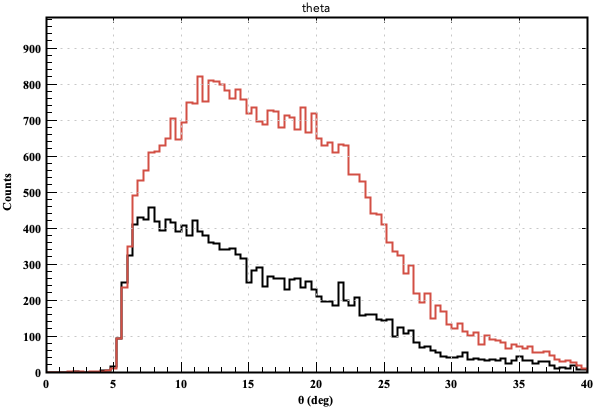
\includegraphics[width=2.0in]{images/pos_theta_5SL.png}
  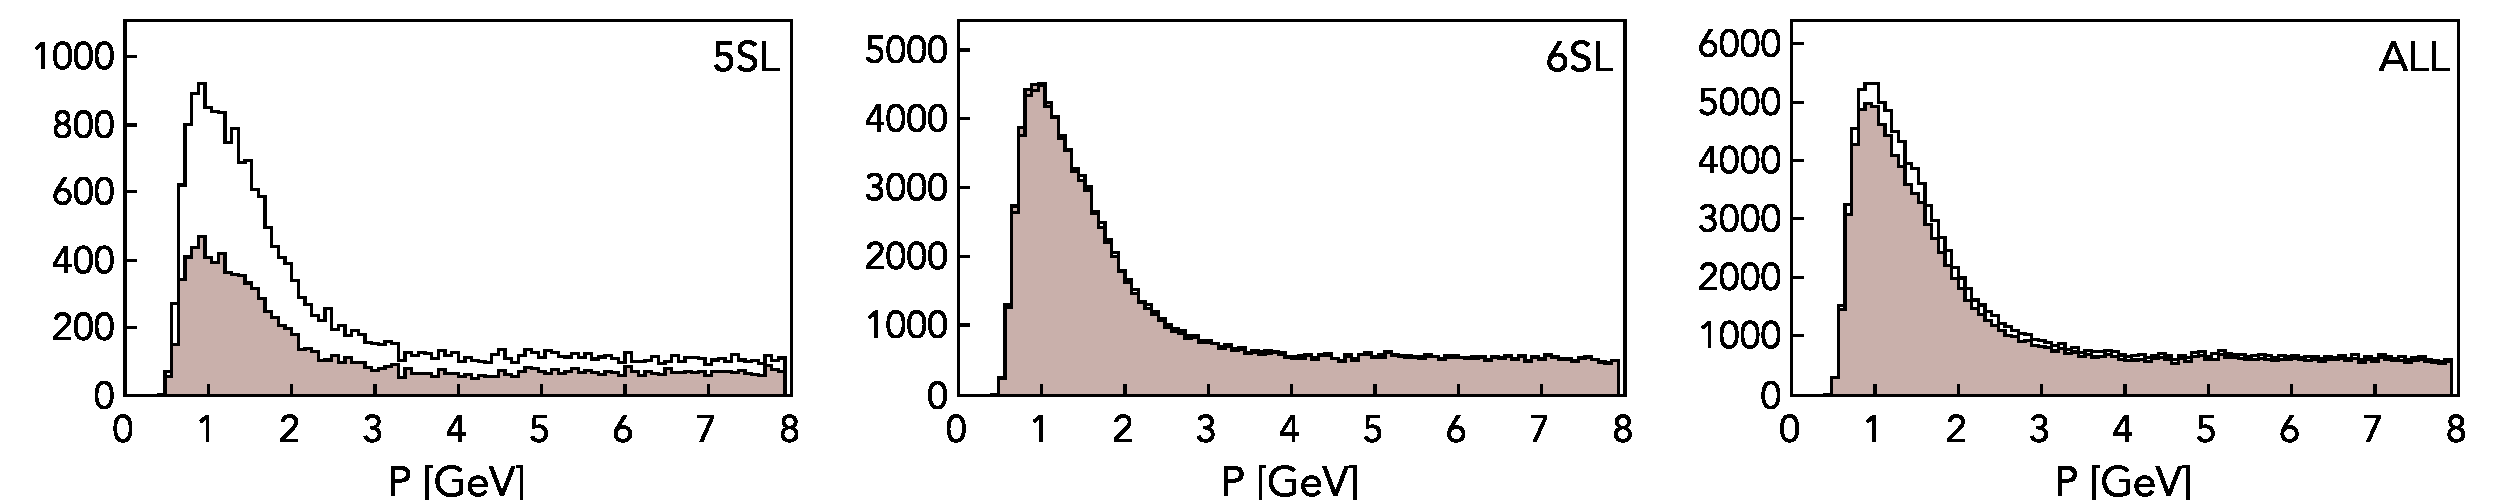
\includegraphics[width=6.5in]{images/figure_p.pdf}
  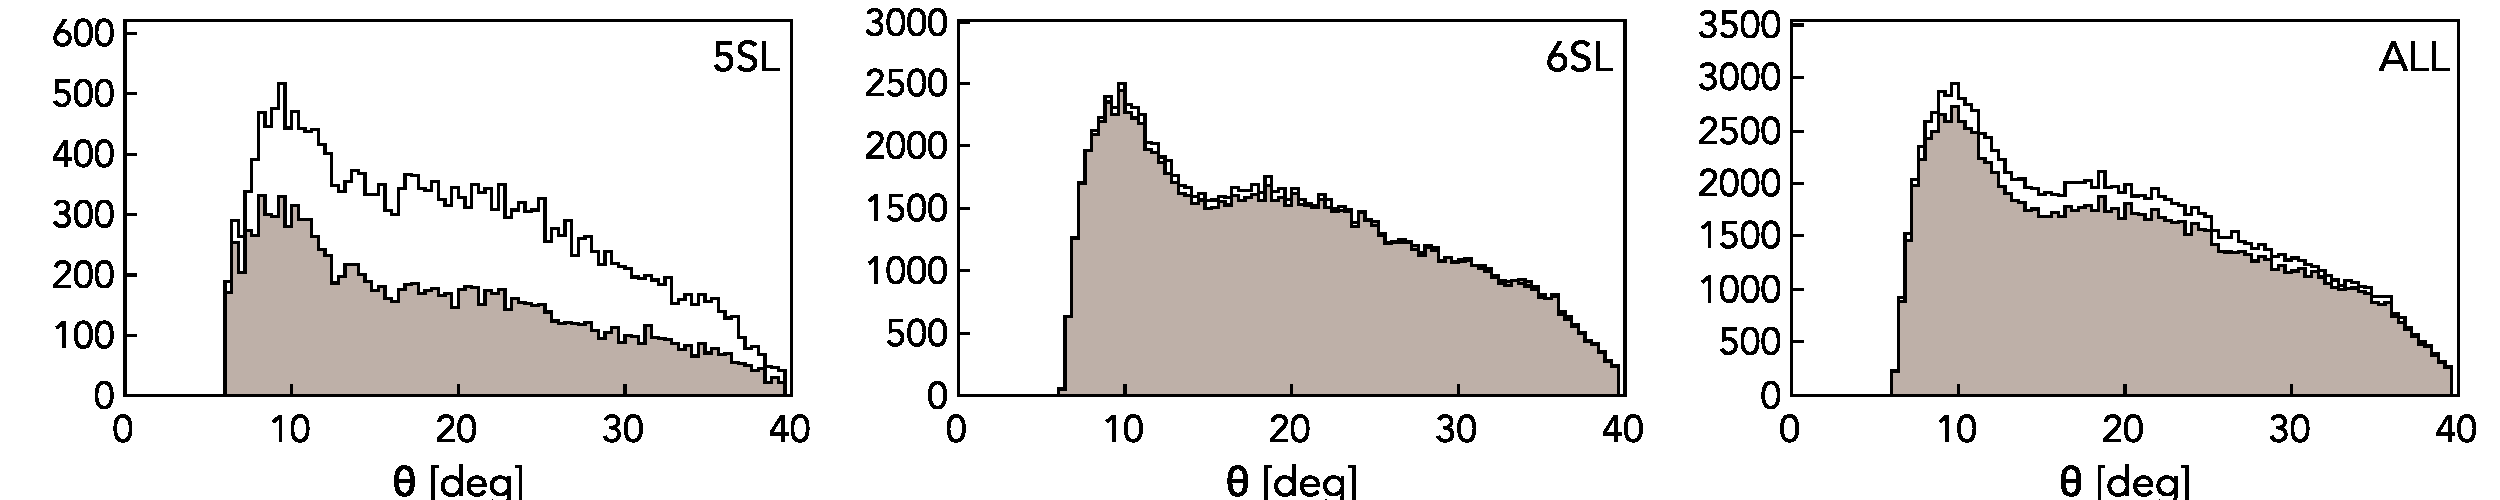
\includegraphics[width=6.5in]{images/figure_theta.pdf}
    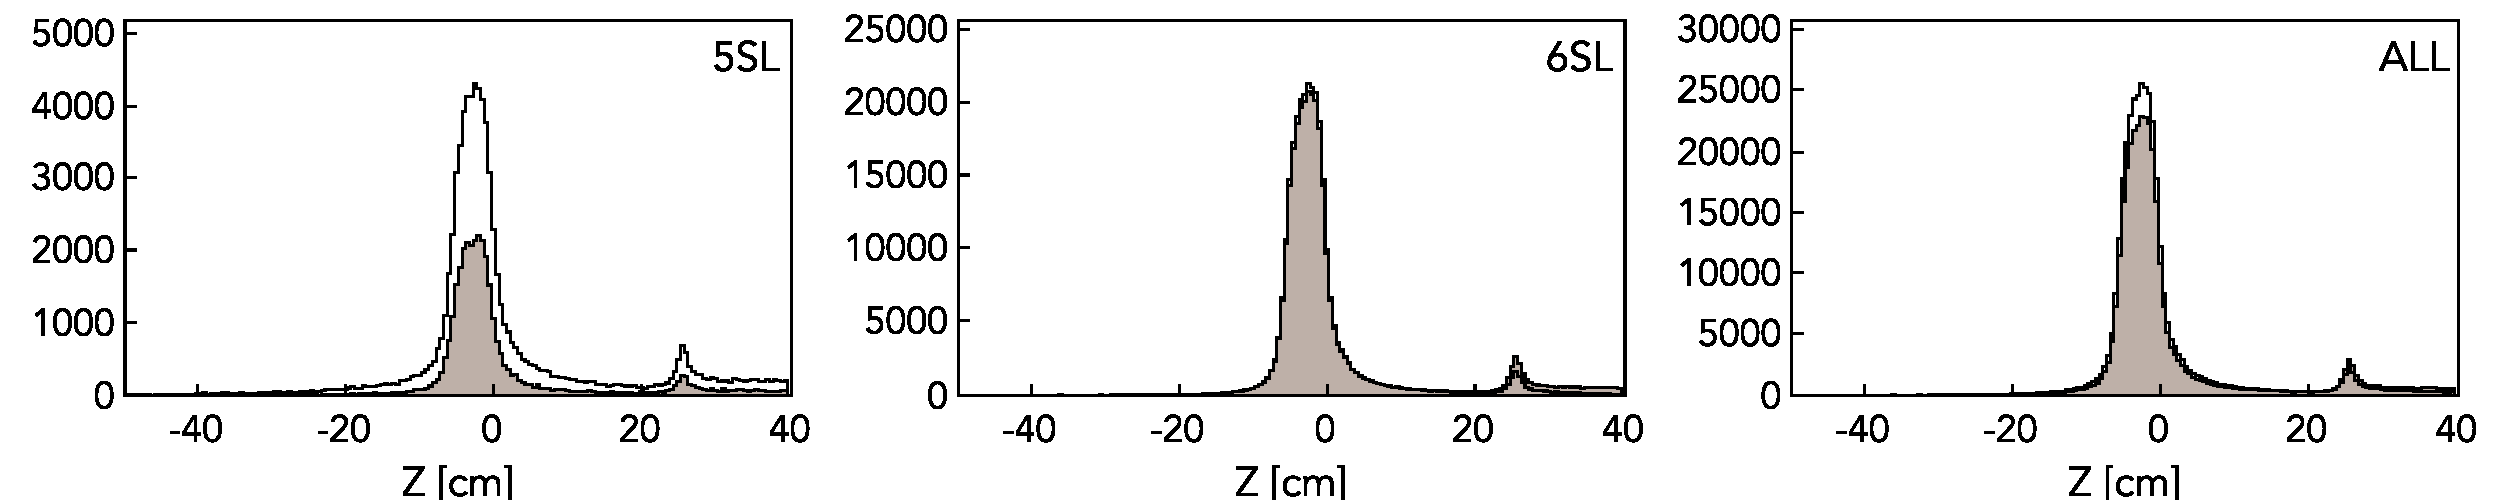
\includegraphics[width=6.5in]{images/figure_vz.pdf}
\caption { Comparison of number of tracks reconstructed with the conventional algorithm vs AI-assisted tracking code as a function of momentum, polar angle and particle interaction vertex. The comparison is shown for 5 super-layer, 6 super-layer tracks (left two columns), and the total number (right column).}
 \label{track:efficiency}
 \end{center}
\end{figure}

The results are shown on Figure~\ref{track:efficiency}, where dependence of number of reconstructed negatively charged 
 tracks are shown as a function of particle momentum (top row), polar angle in laboratory frame (bottom row) and interaction
 vertex (middle row). The reconstructed distributions from conventional tracking are plotted with filled histograms and the
 tracks reconstructed using assistance from AI are plotted with solid lines. As can be seen from the figure, there is a large gain 
 in the number of reconstructed tracks with the 5 super-layer configuration compared to full 6 super-layer tracks. Typically for nominal 
 45 nA experimental data increase in track efficiency for 6 super-layers tracks averages about $3\%-6\%$, while for 5 super-layer
 tracks the increase is in the order of $70\%-120\%$. In normal data reconstruction, tracks that are identified with 5 super-layers
 usually comprise about $10\%$ of all reconstructed tracks, and a significant increase in identification of such tracks leads to 
 overall tracking efficiency increase of $12\%-15\%$. 
 
 \begin{table}[!h]
 \begin{center}
 \begin{tabular}{|l|c|c|c|c|}
 \hline
 Track Configuration & Conventional & AI Assisted & Gain & Relative \\
 \hline
 \hline
 6 Super-Layer & 242,145 & 256,175 & 14030 & 1.0579 \\
 5 Super-Layer & 24,155 & 52,839 & 28684 & 2.1875 \\
 All & 267,339 & 309,058 & 51719 & 1.1561 \\
 \hline
 \end{tabular}
 \end{center}
 \caption{Summary of reconstructed tracks and gain with assistance from Artificial Intelligence.}
 \label{tbl:summary}
 \end{table}
 
The comparison of 5 super-layer and 6 super-layer track statistics and their relative gain is summarized in Table~\ref{tbl:summary}.
As can be seen from the table the gain in only 6 super-layer tracks is about $5.7\%$ but with significant gain in 5 super-layer tracks 
the overall gain in reconstructed tracks elevates to $>15\%$. These results are intuitive since track candidates composed of 5
super-layers with the same number of clusters in each super-layer are significantly higher than 6 super-layer track candidates, and 
in our tests AI performs better in choosing the right combination with increasing combinatorics.
 
\subsection{Luminosity Dependence}

Track reconstruction efficiency increased with AI-assisted tracking, since AI can better identify tracks
from a pool of candidates. One would expect that if the number of combinations decrease the efficiency 
of the conventional track selection algorithm should approach the efficiency of AI-assisted track identification.
Similarly, when the number of combinations increases the advantage of AI over the conventional algorithm should
increase. Based on this we expect AI to perform better in higher background settings. To evaluate AI-assisted
tracking efficiency dependence on background we analyzed several different runs that were taken in different 
conditions (i.e. beam current) ranging from $5~nA$ to $70~nA$. To measure tracking efficiency we first calculated
the number of electrons ($N_e$) detected in the data sample analyzed (typically one run) and then the number of positive and negative
 hadrons that were detected with the electron inclusively ($N_{h^+e}$ and $N_{h^-e}$ respectively).

Then the efficiency for the data set was calculated as:

\begin{equation}
L_t^+ = \frac{N_{h^+e}}{N_e} , L_t^- = \frac{N_{h^-e}}{N_e} 
\end{equation}

where $L_t^+$ is the efficiency of positive particles and $L_t^-$ is the efficiency of negatively charged particles respectively. 
In order to estimate the charged particle reconstruction efficiency as a function of the beam current, the multiplicity, $L_t^{+/-}$, is fitted with a linear function:
\begin{equation}
L_t^{+/-} = a + c\times I 
\end{equation}

Here $a$ and $c$ are the fit parameters and $I$ is the beam current. Then it was assumed that the reconstruction efficiency, $E=1$ at $I=0$ nA:

\begin{equation}
E^{+/-} = 1 + b \times I 
\end{equation}

with $b=\frac{c}{a}$. The slope parameter b is the rate of the reconstruction inefficiency as a function of the beam current \cite{Stepanyan:2020bg}.
%The all points were 
%fitted with linear function $L=a+bx$, where $a$ is the intercept 
 
 \begin{figure}[!ht]
\begin{center}
 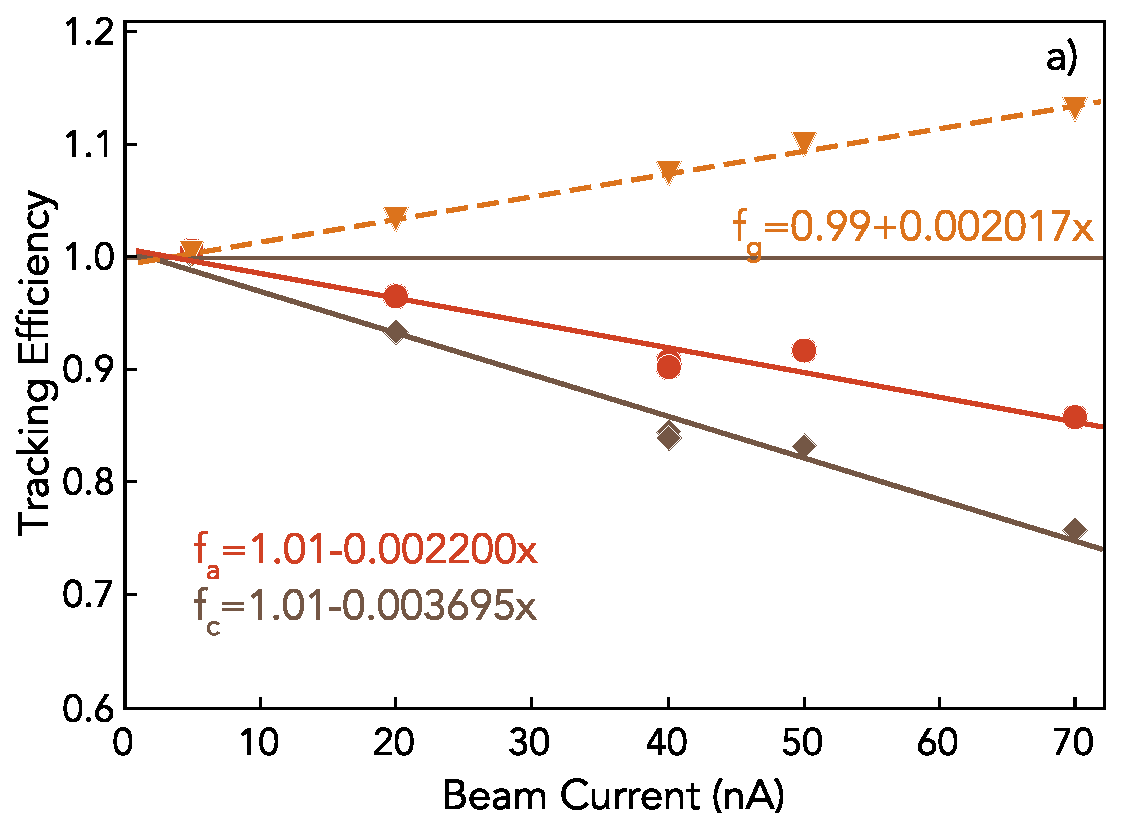
\includegraphics[width=3.0in]{images/figure_lscan_pos.pdf}
 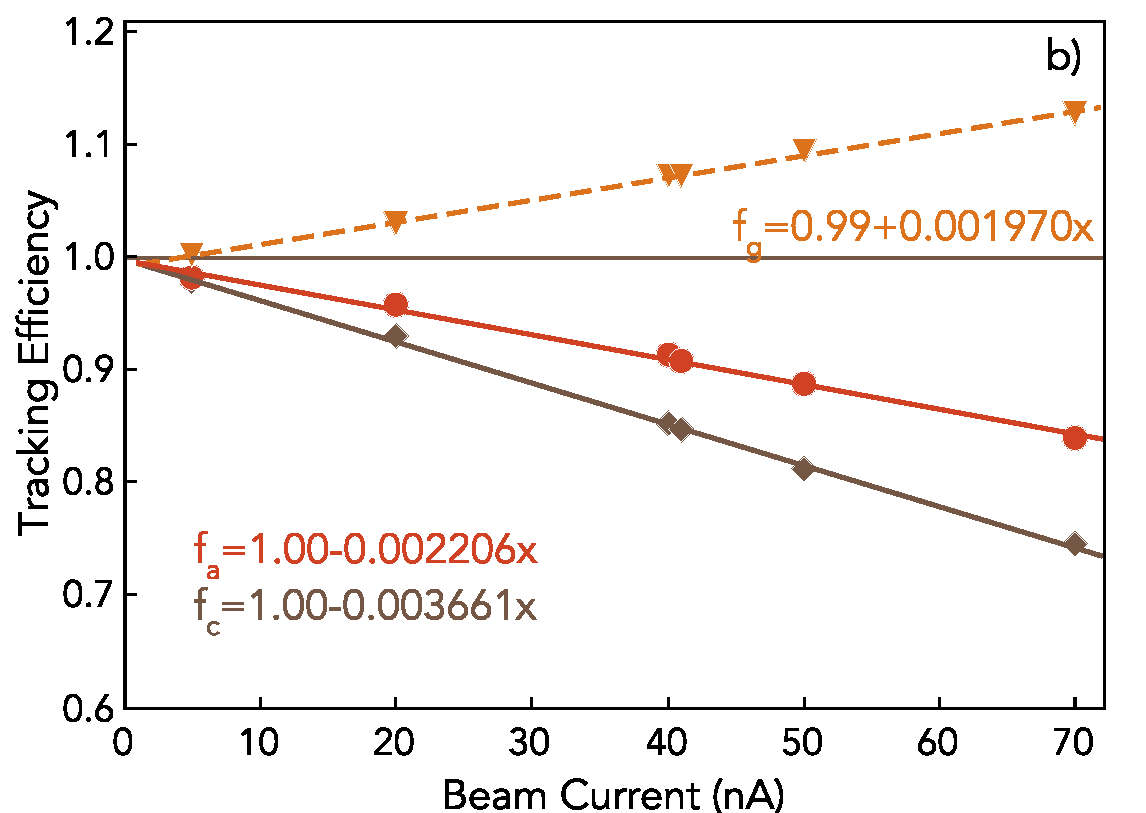
\includegraphics[width=3.0in]{images/figure_lscan_neg.pdf}
\caption {Tracking efficiency for positively and negatively charged particles as a function of beam current (luminosity).  Conventional algorithm 
track reconstruction efficiency (diamonds) is compared to AI-assisted track reconstruction efficiency (circles). }
 \label{lumi:scan}
 \end{center}
\end{figure}

The comparison of tracking efficiency as a function of beam current (luminosity) can be seen on Figure~\ref{lumi:scan} where $E^{+/-}$ are shown for positively and negatively charged particles separately. As can be seen from the figure, AI-assisted tracking performs significantly better for any given luminosity (beam current) and the decrease of efficiency is much slower as a function of luminosity, $0.22\%$ per nA versus $0.40\%$ per nA for conventional tracking. This is expected and consistent with the assumption that with increased combinatorial background (increased number of track candidates to consider), AI performs better in choosing the best track candidate. We established that AI-assisted
tracking leads to more tracks reconstructed for any given beam current setting. The next thing to check is what is the impact of increased track reconstruction efficiency on physics analysis.
% and if there is increase in physics outcome for the CLAS12 experimental setup.

\subsection{Physics Impact}

To measure practical implications of track reconstruction efficiency improvement on physics outcome we analyzed 
two event topologies with two particle and three particles in the final state respectively. The data for analysis were 
taken with $10.5~GeV$ electron beam incident on $20~cm$ liquid hydrogen target, with a beam current of $45~nA$
(typical for CLAS12 experimental running). We selected events where an electron was detected in the forward detector, and 
then isolated events where there was an additional negatively charged pion ($\pi^-$) along with an electron and no other 
charged particle. The second topology required two pions along with electron, one positively charged and one 
negatively charged. The two chosen topologies are denoted by $H(e,e'\pi^-X)$ and $H(e,e'\pi^+\pi^-X)$. In both cases 
there is a visible peak of a missing proton that we can use to measure the impact of efficiency on physics outcome. 

 \begin{figure}[!ht]
\begin{center}
 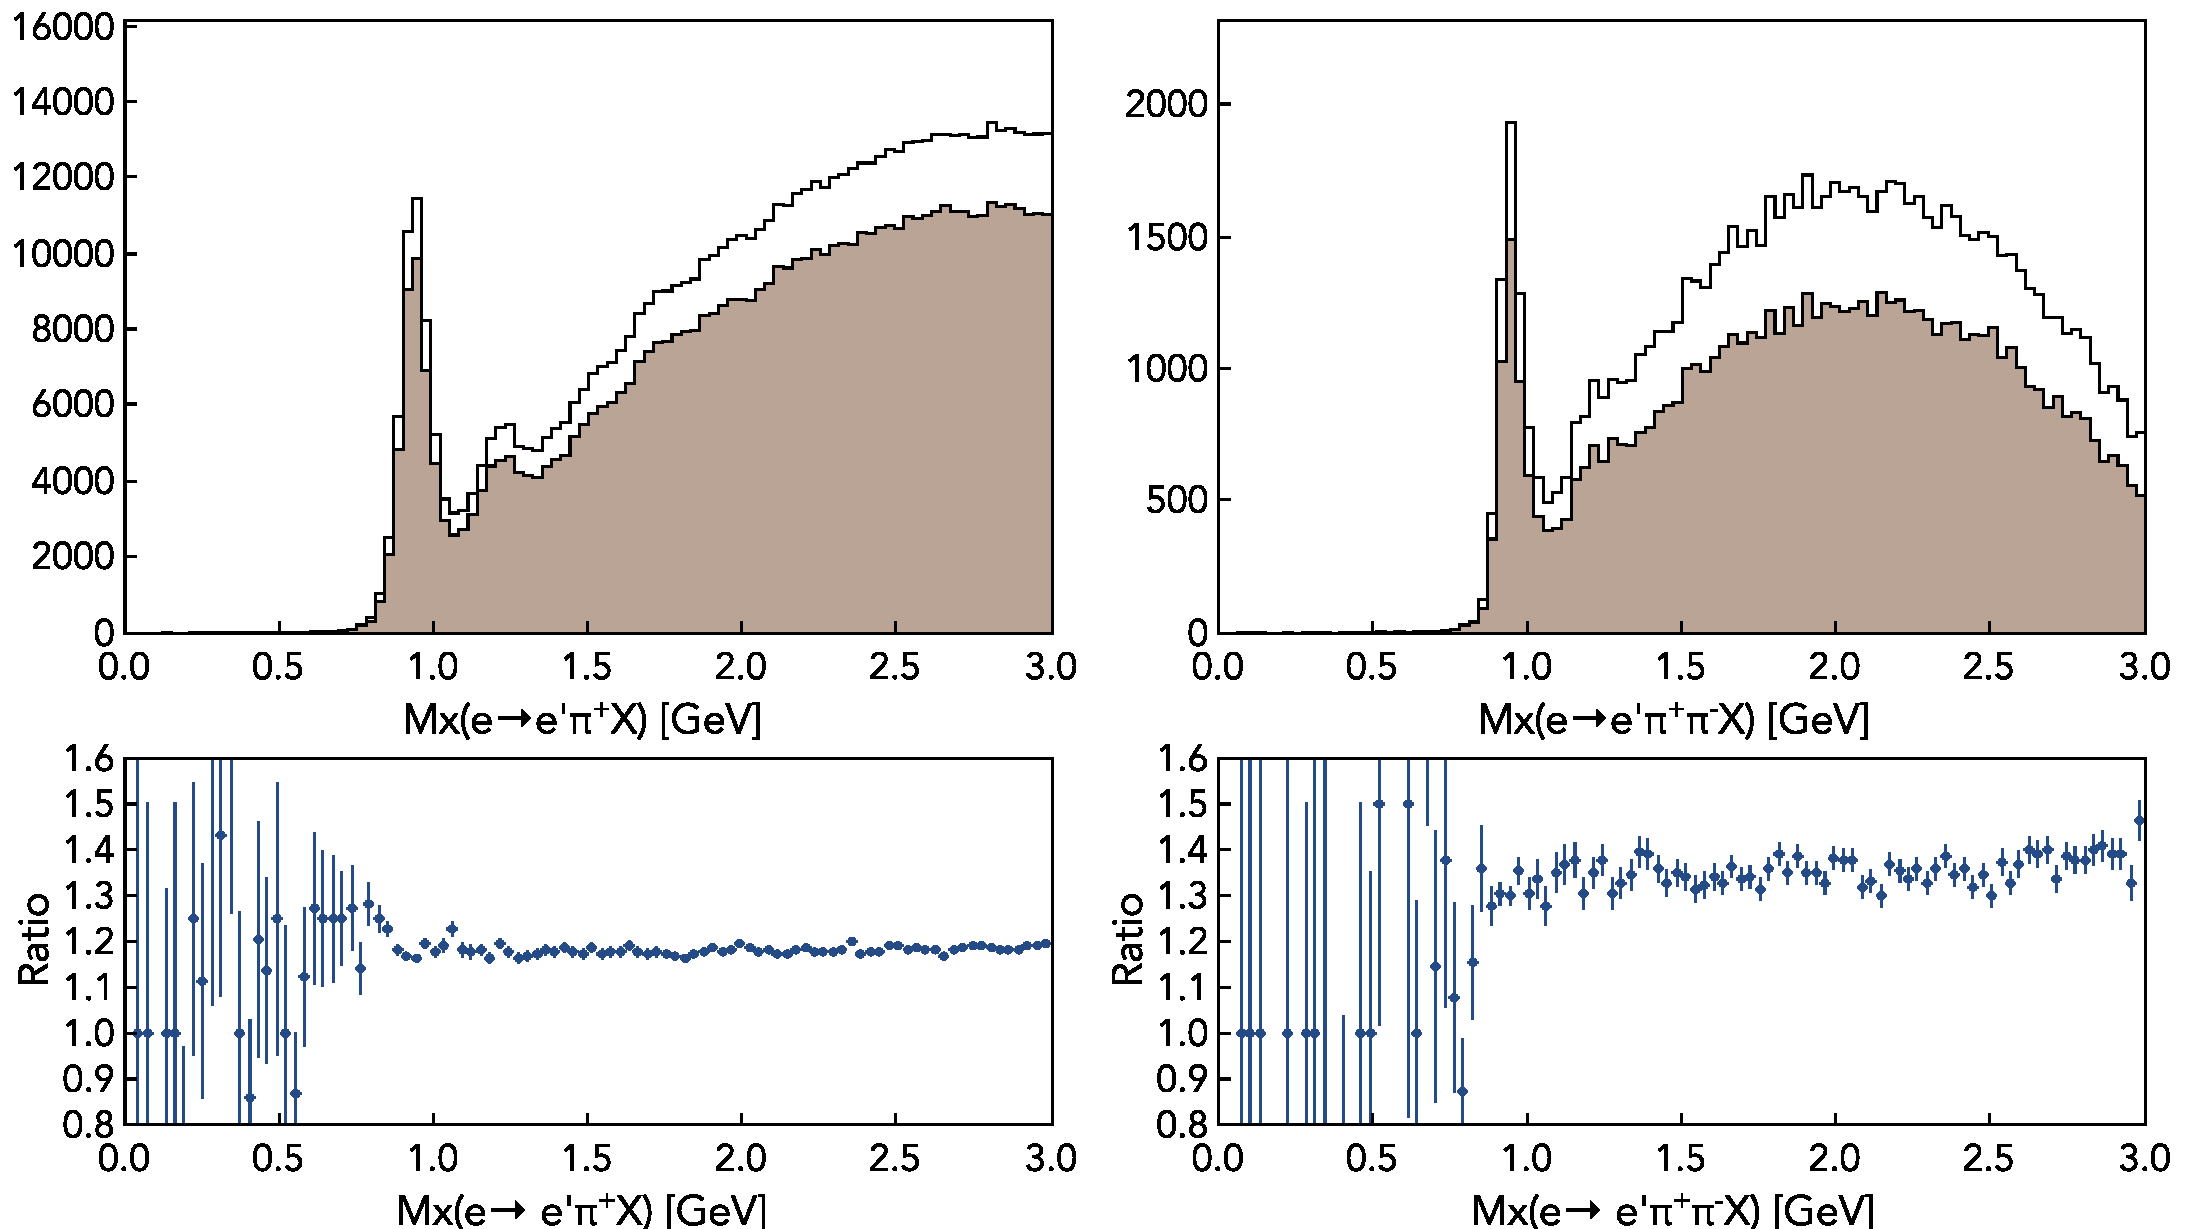
\includegraphics[width=6.0in]{images/physics_scan.pdf}
\caption {Architecture of corruption fixing Auto-Encoder.}
 \label{physics:outcome}
 \end{center}
\end{figure}

The distributions of missing mass for both final state topologies are shown on Figure~\ref{physics:outcome}, where the plots 
on the top row are missing mass of $H(e,e'\pi^-X)$ and $H(e,e'\pi^+\pi^-X)$, where the filled histogram is calculated from 
particles reconstructed by the conventional tracking algorithm, and the histogram with black outline are the same distributions 
calculated from particles that were reconstructed using suggestion from Artificial Intelligence. As can be seen from the figure, 
there is significant increase in the number of events under the missing proton peak (at mass value $0.938~MeV$) for AI assisted
tracking. The ratios of the two histograms (AI-assisted divided by conventional) can be seen on the bottom row of 
Figure~\ref{physics:outcome}. As can be seen from the figure the increase in statistics is uniform over the whole range of the 
missing mass indicating no systematic abnormalities for AI-assisted tracking. The ratio also indicates that there is an increase 
for the number of events under the peak for proton, about $15\%$ for $H(e,e'\pi^-X)$ final state and $30-35\%$ for the $H(e,e'\pi^+\pi^-X)$
final state. Further studies show that improvements in statistics are larger for higher luminosity (incident beam current), which is consistent with our studies of increased efficiency of single particle reconstruction.
%Further studies show that increase in statistics for different final states increase with increase of beam current (luminosity) 
%which is consistent with our studies of increased efficiency of single particle reconstruction. 


\section{Summary}

In this paper we investigated results of analysis of experimental data from CLAS12 detector reconstructed with assistance of Artificial Intelligence
to identify tracks from the hits in drift chambers. This work is based on two neural networks developed to classify track candidates from
given cluster combinations \cite{Gavalian:2020oxg} and to identify missing cluster positions in tracks that do not have complete 6 cluster configuration \cite{Gavalian:2020xmc}. After implementing these networks into the CLAS12 reconstruction workflow, the AI was able to identify "good" track candidates 
and pass them to the tracking code to be analyzed parallel to conventional algorithm that chooses "good" track candidates iteratively considering all possible combinations. 
Our studies showed that AI-assisted tracking performs better than conventional track identification algorithm, and leads to track reconstruction efficiency increase of $15\%$ for nominal experimental running conditions (beam current 45 nA). The AI also performs better with increasing background (i.e. with increased incident beam current) and improves the efficiency loss from $0.44\%$ per nA to $0.24\%$ per nA.
This increased track reconstruction (identification) efficiency directly impacts the outcome of physics analysis where it increases statistics 
for physics reactions for $15\%-35\%$ depending on how many particles are detected in the final state and the topology of the reaction. This has big implication on experimental running conditions, since with increased efficiency the required statistical significance of the experiment can be reached in a shorter time by running at higher beam current (luminosity). Already collected experimental data can be re-processed with the AI-assisted tracking
code which can increase the statistics for analyzed data up to $35\%$. Both, future experiments and already completed ones will benefit 
from this novel development.

Another important outcome of this development was a reduction in data processing times. Since track candidates were identified by AI, there were fewer marginal quality tracks picked to be analyzed and then later dropped due to non-convergence of Kalman filter, leading to tracking code speedup  of $35\%$.

Overall we identified that AI assistance in tracking codes is a good approach, and leads to improvements in code speed and 
efficiency of track reconstruction. Another important aspect of using AI is that is leads to a very small and simple codebase, comprised of composing track candidates and feeding them the the neural networks, and what's also important is that it keeps improving with constant training on new data.
We intend to continue this development in extending the approach to other tracking detectors of CLAS12, and possibly try to adopt  our approach for other experimental detector setups at Jefferson Lab.

